\documentclass[11pt]{article}

% --- Packages ---
\usepackage[margin=1in]{geometry}
\usepackage{amsmath, amssymb}
\usepackage{graphicx}
\usepackage{booktabs}
\usepackage{caption}
\usepackage{float}
\usepackage[hidelinks]{hyperref}
\usepackage{microtype}
\usepackage{enumitem}
\usepackage{multirow}
\usepackage[table]{xcolor}

% --- Spacing / style ---
\setlength{\parskip}{0.5em}
\setlength{\parindent}{0pt}
\captionsetup{font=small, labelfont=bf}

\title{Tailored k-means for Spatial Clustering with Obstacles:\\
A Wildfire Case Study}
\author{Michele Perry}
\date{\today}

\begin{document}
\maketitle

%==============================================================
\begin{abstract}
%==============================================================
Standard k-means groups points by straight-line distance, which is rarely the practical distance between objects in the real world. A lake, a highway, a mountain range, or any other geographic barrier can change how close two points really are. We develop an obstacle-aware version of k-means that adds a single feature, the arc-length position $s$ of each point along a closed obstacle boundary, and weights it against ordinary spatial distance through one tunable parameter $\beta$. Setting $\beta = 0$ recovers standard k-means, so the method is a strict generalization. We apply it to wildfire records from 1992 to 2020 around two lakes of contrasting shape: Lake Tahoe (compact and roughly oval) and Lake Mead (long and narrow with several arms). At the basin scale, both lakes improve by 7 to 8\% in mean shoreline span over standard k-means. Near the shore the lakes diverge: the obstacle parameter does nothing for Tahoe but tightens Mead's clusters by 19\%, the largest gain in the project. The arc-length parameter helps when a lake's shape makes distance along the shore differ sharply from straight-line distance, which compact lakes rarely do and multi-arm lakes do constantly. 
\end{abstract}
 
%==============================================================
\section{Introduction}
%==============================================================
 
\subsection{Motivation}
 
Clustering is one of the most common tools in spatial data analysis. Given a set of points scattered across a region, k-means groups them into $k$ clusters by minimizing distance to a set of centers. The notion of distance is the ordinary straight line between two coordinates, and on open terrain this works well. But the practical distance between two objects in the real world is rarely a straight line. Roads bend around terrain, ecological barriers separate populations, highways and rivers cut neighborhoods in half, and a lake puts water between two points that look close on a map.
 
This matters whenever a clustering result is going to be used. Suppose we are trying to place firefighter stations at central locations for the fire hotspots around a lake. The center of a cluster, in straight-line terms, can sit on the wrong side of the water from many of the fires it nominally represents. The same issue appears in placing disaster response teams near sources of danger, in studying species separated by a physical barrier, in urban planning around major roadways, and in dispersing resources efficiently across a region. In each case, the clustering should reflect distances along travelable paths rather than across barriers. Standard k-means cannot make that distinction. Two points on opposite sides of a lake look as close as two points on the same shoreline.
 
This report develops a version of k-means that addresses the barrier case for a closed boundary curve, and applies it to wildfire data around two lakes. A lake is a useful first case because the obstacle is bounded, has a well-defined shape, and is large enough to genuinely change which points are practically close to which others, but not so large that it carves the surrounding region into entirely separate worlds. Wildfires are a natural choice of point data because they have real safety and resource-allocation stakes: response stations should sit central to where fires actually occur, in terms of driving distance rather than straight-line distance.
 
\subsection{Approach}
 
The fix adds one feature to each point. Alongside its scaled coordinates $(x, y)$, every fire gets an arc-length parameter $s \in [0, 1]$ that records its position along the lake's shoreline, found by projecting the fire onto the boundary and measuring how far around the loop that projection lies. Two fires on the same stretch of shore have similar $s$; two fires on opposite shores have very different $s$, even when their coordinates overlap. The clustering distance combines the two: ordinary straight-line distance plus a weighted term in $s$. A single parameter $\beta$ controls how much the shoreline term counts. At $\beta = 0$ the $s$ term vanishes and the method is exactly standard k-means; as $\beta$ grows, position along the shore carries more weight.

The structural idea -- two kinds of features combined in a tuned non-Euclidean distance -- follows McMahon et al.~\cite{mcmahon2022}. Their tailored self-organizing map clusters U.S. counties using a distance that combines geographic location with disease incidence attributes, with the relative weighting of the two subspaces chosen by optimizing a design objective that rewards clusters showing significant differences in additional demographic variables. They note that the same machinery can be applied to a k-means base, which is what we do here, with a different second feature -- arc-length along an obstacle boundary rather than a vector of attributes -- and a different higher-level objective.
 
The report works through three pieces. A synthetic toy problem isolates what the arc-length parameter does on an obstacle simple enough that the effect is unambiguous. Two case studies apply the method to real wildfire data around lakes of contrasting shape, each at two spatial scales (basin and near-shore). A cross-lake comparison suggests where the method might help and where it might not. The clustering throughout uses location only, with $k = 4$ held fixed across both lakes so that any difference in behavior reflects the lakes' geometry rather than a different number of clusters.

 
%==============================================================
\section{Method}
\label{sec:method}
%==============================================================
 
\subsection{The arc-length parameter}
 
Each point $i$ has scaled planar coordinates $(x_i, y_i)$, obtained by Min-Max scaling longitude and latitude to $[0,1]$, and an arc-length position $s_i \in [0,1]$ along the obstacle boundary. The full feature vector is $\mathbf{x}_i = (x_i, y_i, s_i)$. The obstacle itself is a closed curve $\gamma(t)$, $t \in [0,1]$: in the toy problem it has an exact parametric form, and for the lakes it is a cubic spline fit through the shoreline vertices, closed so that $t = 0$ and $t = 1$ are the same point.
 
To assign a point its arc-length position, project it onto the boundary. The projection of a point $p = (x_p, y_p)$ is
\[
t^*(p) = \arg\min_{t \in [0,1]} \, \big\lVert \, p - \gamma(t) \, \big\rVert^2,
\]
the value of $t$ whose boundary point sits closest to $p$. The raw parameter $t$ is not yet what we want, because equal steps in $t$ do not generally cover equal lengths of a spline: the curve can move more quickly along some stretches of the boundary than others. To get a position that reflects true distance along the shore, we convert $t^*$ to arc length by integrating the local speed of the curve, $\|\gamma'(\tau)\|$, from $0$ up to $t^*(p)$, then normalize by the total perimeter $L$ so that the result lies in $[0,1]$:
\[
s(p) = \frac{1}{L} \int_{0}^{t^*(p)} \big\lVert \gamma'(\tau) \big\rVert \, d\tau,
\qquad
L = \int_{0}^{1} \big\lVert \gamma'(\tau) \big\rVert \, d\tau.
\]
With this normalization, equal steps in $s$ cover equal stretches of shoreline, so two points on the same stretch of shore have similar $s$, while two points on opposite sides of the obstacle have very different $s$, even when their coordinates are close.
 
Because the boundary is a closed loop, $s = 0$ and $s = 1$ are the same location, and distance in $s$ has to respect the seam. The loop-aware distance measures the shorter way around:
\begin{equation}
d_s(s, s') = \min\!\big(\, |s - s'|, \; 1 - |s - s'| \,\big),
\label{eq:loop-distance}
\end{equation}
which correctly gives $d_s(0.99, 0.01) = 0.02$ and reaches its maximum of $0.5$ when two points sit on opposite sides of the loop.

\subsection{Obstacle-aware k-means}
 
Obstacle-aware k-means keeps the structure of standard k-means -- alternate between assigning points to the nearest centroid and updating centroids -- but changes the distance used in the assignment step. For a point $\mathbf{x} = (\text{geo}, s)$ and a centroid $\boldsymbol{\mu} = (\text{geo}_\mu, s_\mu)$,
\begin{equation}
d^2(\mathbf{x}, \boldsymbol{\mu})
= \alpha^2 \, \big\lVert \text{geo} - \text{geo}_\mu \big\rVert^2
\; + \; \beta^2 \, d_s(s, s_\mu)^2 .
\label{eq:composite}
\end{equation}
The first term is the usual squared straight-line distance between scaled coordinates. The second is the squared loop-aware distance along the shore, weighted by $\beta$. Only the ratio of $\alpha$ to $\beta$ matters, so we fix $\alpha = 1$ and let $\beta$ be the single dial. At $\beta = 0$ the shoreline term disappears and \eqref{eq:composite} is the squared Euclidean distance of standard k-means, so the method is a strict generalization. As $\beta$ grows, position along the shore counts for more, and the clustering increasingly groups fires that share a stretch of shoreline. The method also admits an optional third term for non-spatial attributes, weighted by a parameter $\gamma$; this is set to zero throughout the present report (see Section~\ref{sec:method-refine}).
 
The update step for each centroid takes a small modification on the $s$ component. The planar part is the ordinary mean of cluster members,
\[
(x_{\mu_c},\, y_{\mu_c}) = \frac{1}{|C_c|} \sum_{i \in C_c} (x_i,\, y_i),
\]
but the arc-length part cannot be averaged directly without misbehaving at the seam. Instead we compute it by projecting the planar mean back onto the boundary:
\[
s_{\mu_c} = s\big( (x_{\mu_c}, y_{\mu_c}) \big).
\]
The centroid's shoreline position is then the arc length of its mean location, consistent with how points get their $s$ values in the first place.

The algorithm iterates these assignment and update steps to convergence. We seed it with a variant of k-means++ adapted to the same composite distance: the first centroid is drawn uniformly at random, and each subsequent centroid is sampled with probability proportional to the squared $d^2$ in \eqref{eq:composite} from the nearest existing centroid.
 
\subsection{The arc-length span: measuring shoreline tightness}
\label{sec:span}
 
The headline question is whether obstacle awareness produces clusters that group fires tightly along the shore. The arc-length span measures exactly that, one cluster at a time. Take a cluster's fires and their positions $s$ on the loop $[0,1]$. Sort them and look at the gaps between consecutive positions, including the wraparound gap from the largest $s$ back to the smallest. The largest of these gaps is the widest empty stretch of shoreline the cluster leaves uncovered. The span is what remains once that gap is removed:
\begin{equation}
\text{span}(C_c) = 1 - \max(\text{gaps between consecutive sorted } s \text{ on the loop}).
\label{eq:span}
\end{equation}
This is the length of the shortest arc of shoreline containing all of the cluster's fires, as a fraction of the full loop.
 
The main metric for a whole clustering is the mean arc-length span, averaged over the $k$ clusters, where lower values indicate tighter shoreline grouping. Every comparison in the case studies reports this number against the standard k-means baseline as a percent improvement:
\[
\text{improvement} = 100 \times \frac{\overline{\text{span}}_{\text{standard}} - \overline{\text{span}}_{\text{method}}}{\overline{\text{span}}_{\text{standard}}},
\]
so standard k-means is $0\%$ by definition and a positive number means tighter clusters.
 
\subsection{The objective \texorpdfstring{$J$}{J} and choosing \texorpdfstring{$\beta$}{beta}}
\label{sec:objective}
 
Although the span measures shoreline tightness, minimizing it directly can produce strained clusters that ignore straight-line geography. Instead we tune $\beta$ using the objective $J$, the mean within-cluster distortion:
\begin{equation}
J = \frac{1}{k} \sum_{c=1}^{k} \frac{1}{|C_c|} \sum_{i \in C_c}
\Big( \big\lVert \text{geo}_i - \text{geo}_{\mu_c} \big\rVert^2 + d_s(s_i, s_{\mu_c})^2 \Big).
\label{eq:objective}
\end{equation}
The inner sum averages each cluster's squared distances to its own centroid, combining the straight-line and loop-aware terms; the outer sum averages over the $k$ clusters. Note that $\beta$ does not appear in $J$: the fitting distance \eqref{eq:composite} carries $\beta$, but the scoring distance fixes unit weights so the values are comparable across the whole sweep.
 
\paragraph{Selection procedure.}
We sweep a grid of $30$ values of $\beta$, fit the model at each, and record both $J$ and the mean span. The lowest-$J$ point on the grid is not taken automatically, because $J$ is often nearly flat across a wide range of $\beta$ and an outright minimum can be an isolated numerical spike rather than a meaningful best. Instead we select among the values that pass three filters, then break the tie with span:
\begin{enumerate}[nosep, leftmargin=1.4em]
\item \textbf{Low $J$.} The value's $J$ is within a small tolerance of the grid minimum.
\item \textbf{Stable.} At least one neighboring grid point is also low-$J$.
\item \textbf{No tiny clusters.} Every cluster holds more than $10$ fires.
\end{enumerate}
Among the values that pass, the one with the smallest mean span is selected.

%==============================================================
\section{Toy Problem: A Synthetic Ellipse}
\label{sec:toy}
%==============================================================
 
Before applying the method to wildfire data, it helps to see what the arc-length parameter does on a problem simple enough that the answer is unambiguous. A synthetic ellipse, with three small groups of points placed around it, serves that purpose. The obstacle is geometrically clean, the ``true'' clusters are known by construction, and the only thing that varies between the two methods is the distance they use. If $s$ works as designed, the obstacle-aware version will recover the true grouping while standard k-means fails.
 
\subsection{Setup}
 
The obstacle is the level set of a 2D Gaussian at threshold $c$. Setting
\[
A \exp\!\left( -\frac{(x-h)^2}{2\sigma_x^2} - \frac{(y-k)^2}{2\sigma_y^2} \right) = c
\]
and rearranging gives an ellipse centered at $(h, k)$ with semi-axes $a = \sigma_x \sqrt{-2 \ln(c/A)}$ and $b = \sigma_y \sqrt{-2 \ln(c/A)}$. The parameters $\sigma_x = 3$, $\sigma_y = 0.6$, $h = k = 0$, $A = 1$, $c = 0.01$ produce a long, thin ellipse with a 5:1 aspect ratio (semi-axes 9.10 and 1.82, perimeter $L \approx 38.3$). The ellipse is parameterized as $(\sigma_x \sqrt{-2 \ln(c/A)} \cos t, \sigma_y \sqrt{-2 \ln(c/A)} \sin t)$ for $t \in [0, 2\pi]$, starting at the rightmost tip and increasing counter-clockwise.
 
Fifteen points are placed outside the ellipse in three groups of five, with small Gaussian jitter added to prevent a perfectly regular layout: a northeast group above the right half of the ellipse, a southeast group below the right half, and a west group near the left tip (see Figure~\ref{fig:toy-s}). The northeast and southeast groups overlap in $x$ but sit on opposite sides of the obstacle. Near the right end where the ellipse narrows, points from the two groups can be very close in straight-line distance even though the obstacle separates them. This is the case standard k-means is built to mishandle.
 
\subsection{Standard k-means fails as expected}
 
Running standard k-means (initialized by k-means$++$) with $k = 3$ on the raw $(x, y)$ coordinates produces three clusters, one with a misclassified point. The rightmost southeast point, near $(7.7, -1.3)$, gets pulled into the northeast cluster. In straight-line distance it really is closer to the northeast group's right edge than to the rest of its own group around the left side of the obstacle. Standard k-means has no way to see that the ellipse sits between them, so it makes the assignment the metric dictates. Fourteen of fifteen points end up correctly assigned, but the one that doesn't is exactly the point the geometry would predict.
 
\subsection{The arc-length parameter on this problem}
 
To add the arc-length parameter, project each point onto the ellipse and compute $s$ as described in Section~\ref{sec:method}. The values trace the loop counter-clockwise from the rightmost tip: the north-east points get $s$ between roughly $0.05$ and $0.22$, the south-east points between roughly $0.77$ and $0.95$, and the west points sit near $s = 0.5$. The two groups whose $(x, y)$ values overlap, north-east and south-east, are now cleanly separated in $s$: a point at $s = 0.08$ and a point at $s = 0.92$ are at the maximum loop distance of $0.5$ apart, exactly the kind of separation the new feature was designed to encode.
 
\begin{figure}[H]
\centering
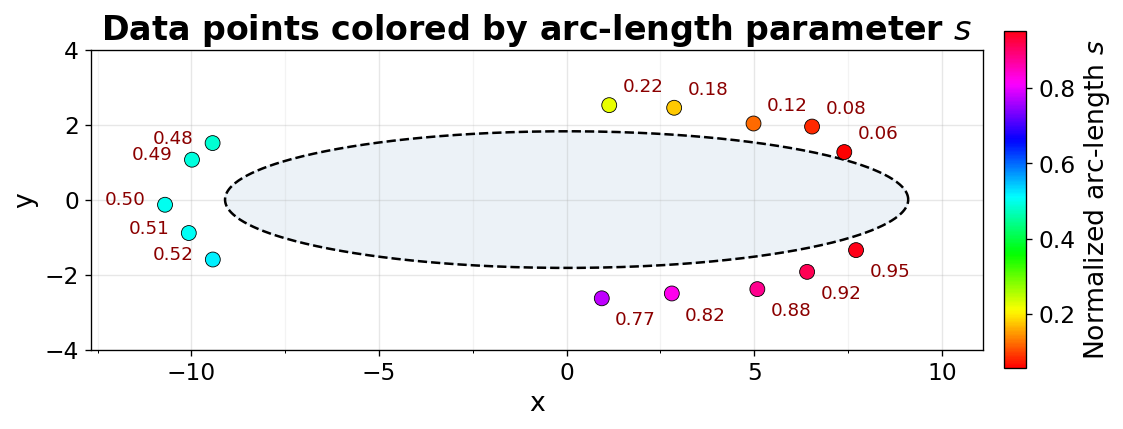
\includegraphics[width=\textwidth]{figures/toy_s_coloring.png}
\caption{Points colored by arc-length position $s$, with the ellipse boundary as a dashed line. The HSV colormap wraps from red back to red across the seam at $s = 0$, reflecting that the boundary is a closed loop. Points on opposite sides of the obstacle take very different colors even when their $(x, y)$ values overlap; west points sit at the maximum separation, near $s = 0.5$.}
\label{fig:toy-s}
\end{figure}

 
\subsection{Obstacle-aware k-means recovers the true grouping}
 
The feature vector for each point is $(x_{\text{scaled}}, y_{\text{scaled}}, s)$, with $(x, y)$ Min-Max scaled to $[0, 1]$ so that all three components live on a comparable scale. After initializing with the tailored k-means++, run obstacle-aware k-means with $k = 3$ and weights $\alpha = \beta = 1$. This clustering assigns the misclassified point correctly: the south-east cluster recovers all five of its members, and the other two clusters also match their ``true'' assignments (see Figure~\ref{fig:toy-comparison}).
 
\begin{figure}[H]
\centering
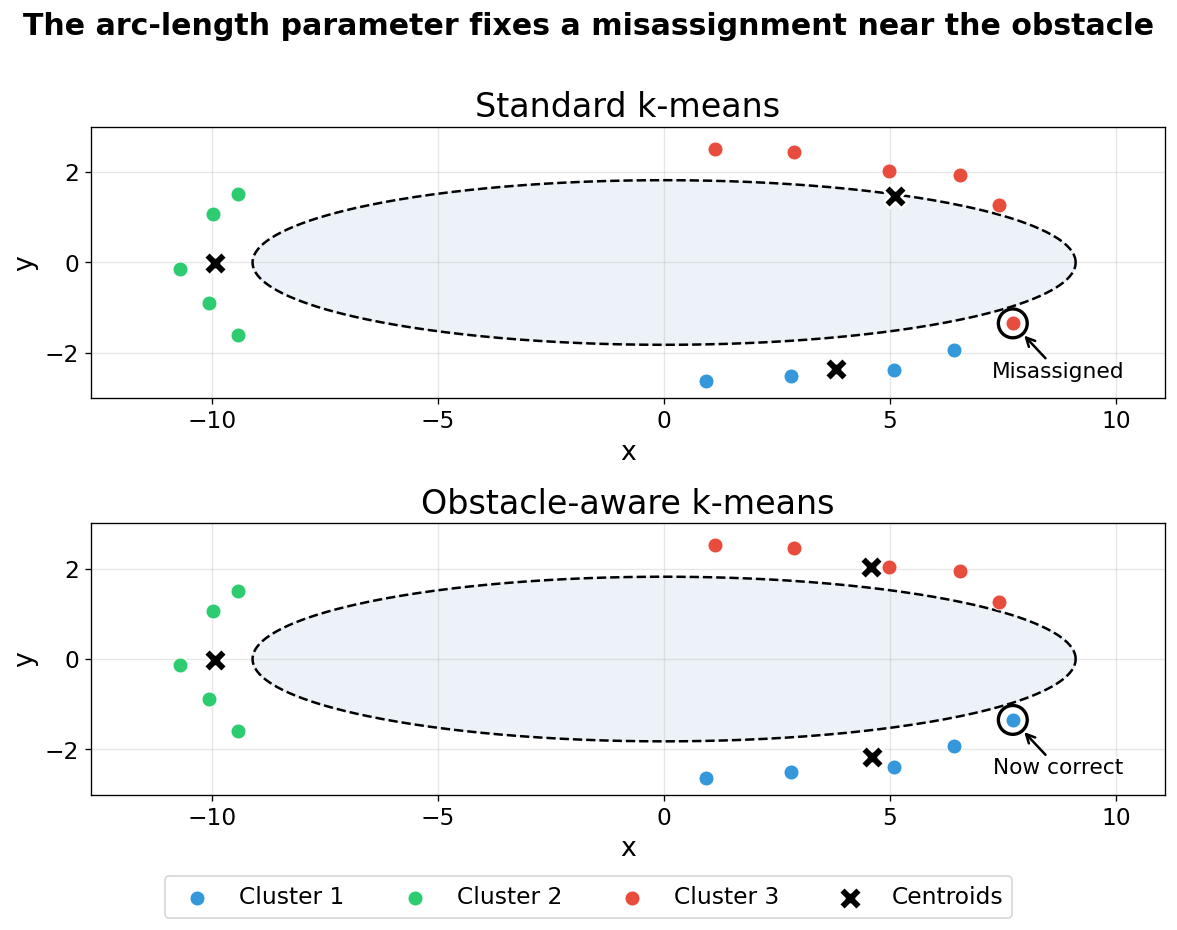
\includegraphics[width=\textwidth]{figures/toy_comparison.png}
\caption{Standard k-means (top) misassigns one point at the right tip of the ellipse, where straight-line distance pulls a south-east point into the north-east cluster. Obstacle-aware k-means (bottom) recovers the correct grouping. The two algorithms differ only in their distance metric; the data, the number of clusters, and the initialization scheme are identical.}
\label{fig:toy-comparison}
\end{figure}
 
\subsection{What this shows, and what it doesn't}
 
The toy problem demonstrates that the arc-length parameter does what it was designed to do: when straight-line distance assigns a point to the cluster on the other side of an obstacle, $s$ pulls it back, and the clustering follows. What the toy cannot do is tell us how much obstacle awareness will help on real data, where the obstacle has a more complicated shape, the points are more numerous and less neatly arranged, and the ground truth is not known. For that we turn to real wildfires and lakes, with a way to score the result that does not depend on knowing the assignments in advance. Section~\ref{sec:tahoe} describes the first case study, Lake Tahoe.

%==============================================================
\section{Case Study: Lake Tahoe}
\label{sec:tahoe}
%==============================================================
 
Lake Tahoe sits on the California-Nevada border in the Sierra Nevada, a single roughly oval basin about 35 km long and 19 km wide. Tahoe makes a good test case because is one closed body of water with a compact shape and a well-defined regulatory boundary around it for selecting fires. The analysis runs at two scales: the basin scale uses every fire inside the Tahoe basin boundary (1,068 fires over 28 years), and the near-shore scale uses only the fires within 1 km of the shoreline.

\subsection{Data and boundary}
 
The fire records come from the FPA FOD~\cite{fpafod}, a USDA Forest Service dataset covering US wildfires from 1992 to 2020. A bounding-box query around the Tahoe area returned 1,888 fires; restricting to those falling inside the official TRPA basin polygon~\cite{trpa} left 1,376. After dropping records whose cause is missing or undetermined (to keep the attribute analysis in Section~\ref{sec:attributes} on a consistent row set), 1,068 fires remained. Each fire's cause was encoded as a binary (Natural / lightning vs.\ Human-caused), and fire size was log-transformed because the raw distribution is severely right-skewed (median 0.1 acres, mean 10.4, maximum 4,222).
 
The shoreline polygon comes from the USGS National Hydrography Dataset~\cite{nhd}, layer 10 (small-scale waterbodies). NHD returned the lake at 1,528 vertices, including a region with dense, narrow channels. Those channels add detail at a scale finer than the cluster boundary needs, so vertices inside the region were dropped (246 vertices removed, 1,282 retained), and the remainder was simplified with Douglas-Peucker at a tolerance of about 100 m. The result is a 269-vertex polygon that preserves the lake's overall shape. A cubic spline fit through those vertices gives the smooth, closed boundary curve $\gamma(t)$ that the method needs for projection. The resulting perimeter is 118.3 km, so a mean arc-length span of $s$ corresponds to roughly $118.3 \times s$ km of shoreline.
 
\subsection{Projecting fires onto the shoreline}
 
Each of the 1,068 fires is projected onto the boundary spline using the procedure from Section~\ref{sec:method}, yielding both its spline parameter $t$ and its arc-length position $s \in [0,1]$. The full range of $s$ is covered, $0.007$ to $0.998$, so the fires touch essentially every stretch of shoreline.
 
\begin{figure}[H]
\centering
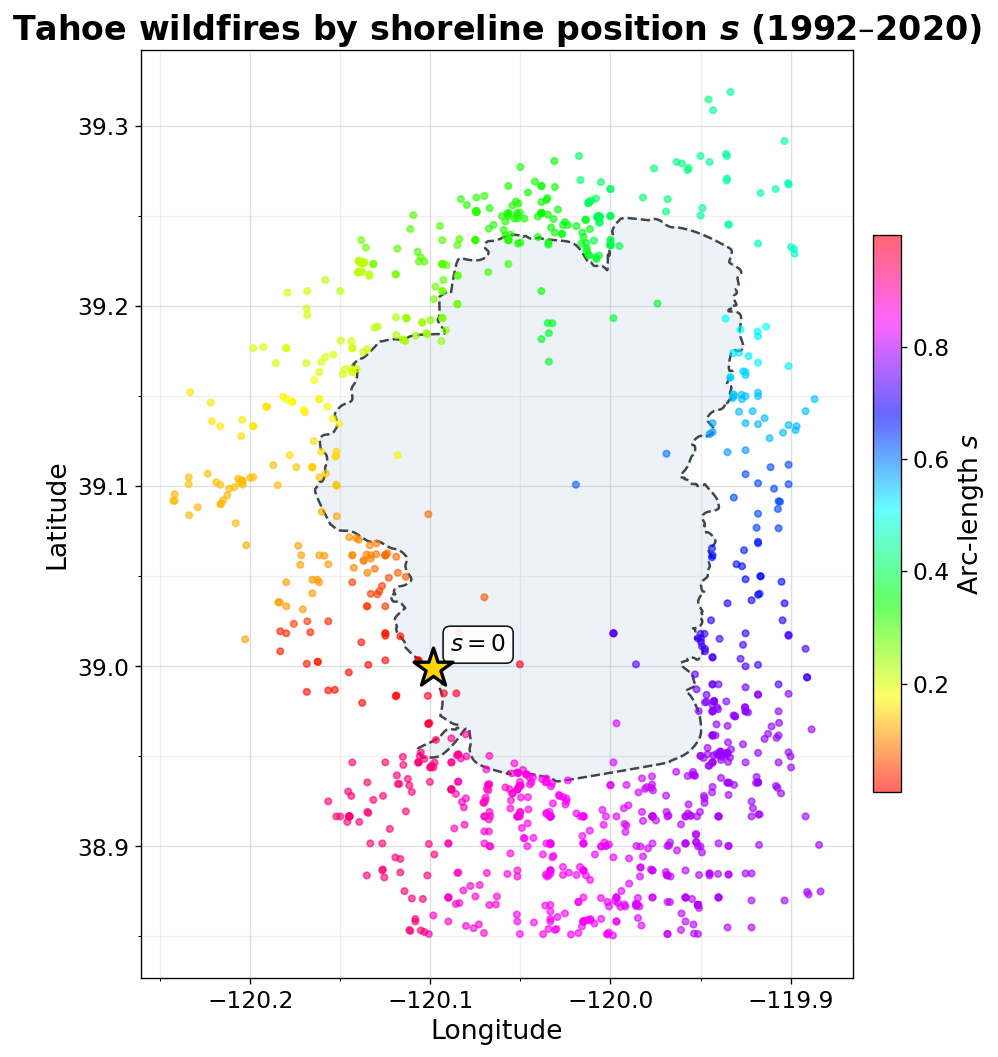
\includegraphics[width=0.8\textwidth]{figures/tahoe_fires_by_s.png}
\caption{Lake Tahoe wildfires (1992--2020) colored by arc-length position $s$ along the shoreline. The HSV colormap wraps from red back to red across the seam at $s = 0$, reflecting the closed loop. Fires are distributed around the entire basin, with $s$ values covering the full range.}
\label{fig:tahoe-s}
\end{figure}
 
\subsection{Choosing the number of clusters}
 
The number of clusters $k$ is held fixed across both lakes for a controlled comparison. The value $k = 4$ comes from the elbow method run on Tahoe's basin coordinates, sweeping $k$ from 2 to 8 and plotting the inertia (within-cluster sum of squared distances) at each.
 
\begin{figure}[H]
\centering
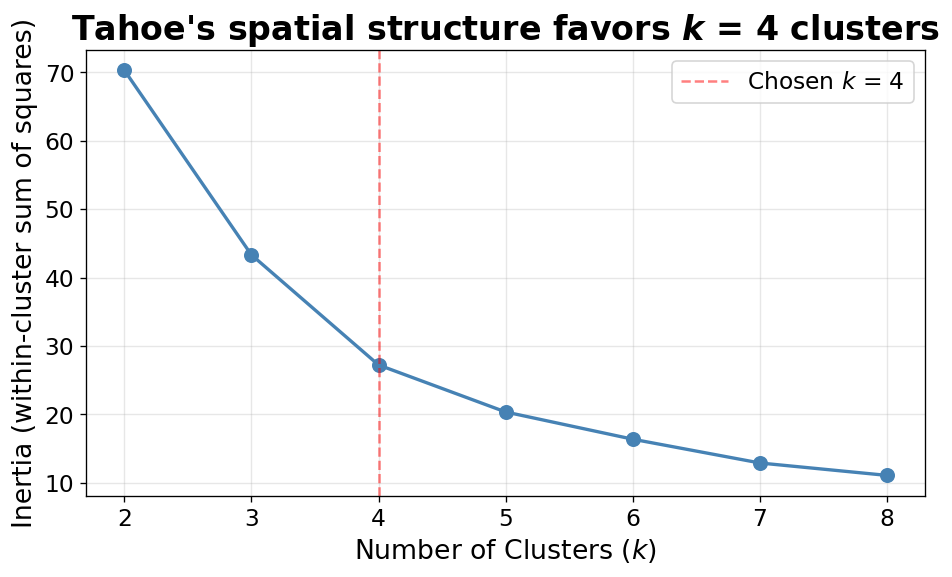
\includegraphics[width=0.9\textwidth]{figures/tahoe_elbow.png}
\caption{Elbow plot for choosing $k$ on Lake Tahoe basin fires. The inertia (within-cluster sum of squared distances) drops sharply through $k = 4$ and flattens afterward, indicating that four clusters capture most of the spatial structure. The same $k = 4$ is used throughout, including the Lake Mead analysis.}
\label{fig:tahoe-elbow}
\end{figure}
 
\subsection{Basin scale: three methods}
\label{sec:tahoe-basin}
 
Three clusterings are run on the full basin of 1,068 fires, each producing four clusters: standard k-means as the baseline ($\beta = 0$), obstacle-aware k-means at equal weights ($\beta = 1$), and obstacle-aware k-means at an optimized $\beta$ chosen by the procedure described below. The headline metric for each is the mean arc-length span, defined in Section~\ref{sec:span}.
 
\paragraph{Standard k-means (baseline).}
Standard k-means on scaled $(x, y)$ converges in 10 iterations and produces four spatially compact clusters with sizes 305, 230, 223, and 310 fires. The mean arc-length span is $\overline{\text{span}}_{\text{std}} = 0.2650$, or about 31.3 km of shoreline per cluster on average. This is the number every obstacle-aware variant is measured against.
 
\paragraph{Obstacle-aware at equal weights.}
Adding $s$ as a clustering feature with $\beta = 1$ converges in 13 iterations and produces a clustering of broadly similar shape: cluster sizes shift slightly to 305, 236, 216, and 311. The mean span drops to $0.2475$ (about 29.3 km), an improvement of $6.6\%$ over standard k-means. Although equal weights is not a tuned choice, it already extracts most of what the obstacle parameter has to offer at this scale.
 
\paragraph{Obstacle-aware at optimized $\beta$.}
The $\beta$ sweep runs the model at 30 values of $\beta$ from 0.05 to 2.5, recording both the objective $J$ and the mean span at each. Figure~\ref{fig:tahoe-basin-sweep} shows the two on a shared $\beta$ axis.
 
\begin{figure}[H]
\centering
\makebox[\textwidth]{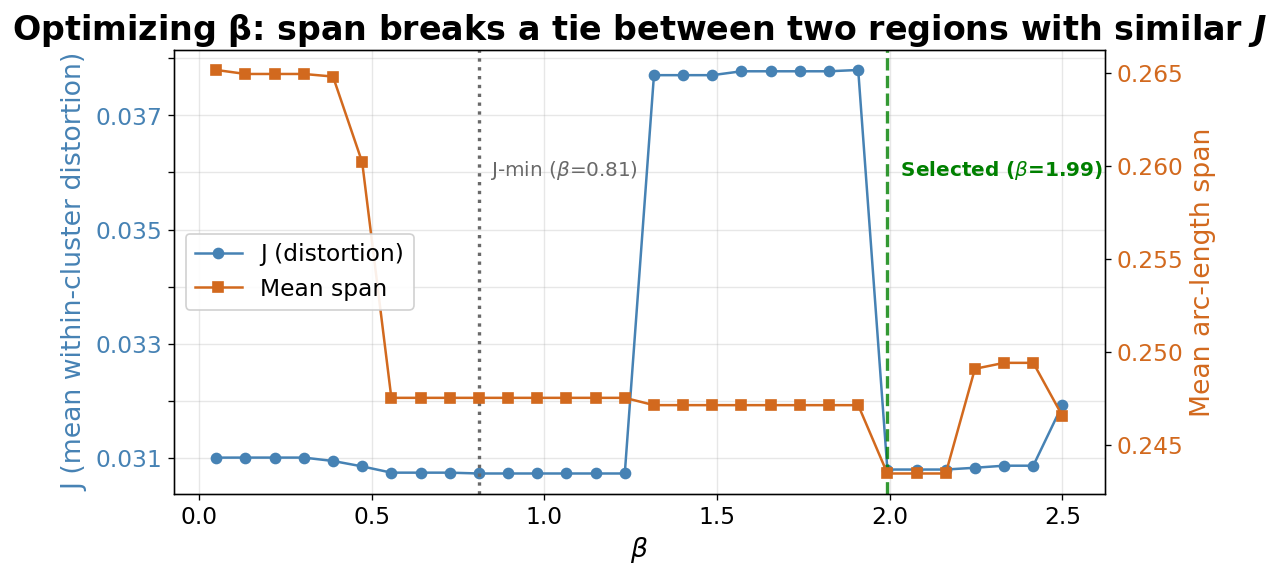
\includegraphics[width=1.1\textwidth]{figures/tahoe_basin_beta_sweep.png}}
\caption{Tahoe basin: $J$ and mean span across the $\beta$ grid. $J$ sits low in two separate stretches with a small ridge between them, so the objective alone does not pin down a single best $\beta$. The selection procedure breaks the tie with span, landing at $\beta \approx 1.99$ in the upper stable region.}
\label{fig:tahoe-basin-sweep}
\end{figure}
 
The selection picks $\beta = 1.99$. The lowest $J$ on the grid sits at $\beta = 0.81$, but $J$ is nearly flat across two separate stretches (one around $\beta \approx 0.8$, another around $\beta \approx 2.0$), with a small ridge between them. In the flat regions, many clusterings are close to equally compact, so $J$ does not single one out. The selection procedure from Section~\ref{sec:objective} restricts to $\beta$ values whose $J$ is within tolerance of the minimum and that have at least one neighboring grid point also low-$J$ (so the choice is stable and not an isolated spike), then breaks ties on span. The upper stable region reaches the lowest mean span on the grid, so $\beta = 1.99$ wins. Every cluster has more than 10 fires, so the cluster-size filter is satisfied automatically.
 
Refitting at $\beta = 1.99$ gives cluster sizes 307, 236, 311, and 214, and a mean span of $0.2435$ (about 28.8 km). That is an $8.1\%$ improvement over standard k-means, a small additional gain on top of equal weights. In absolute terms, the average cluster's shoreline footprint tightened from 31.3 km to 28.8 km -- a 2.5 km decrease, modest in scale.
 
\paragraph{Comparison.}
Figure~\ref{fig:tahoe-basin-compare} shows the three clusterings side by side, with cluster colors aligned across panels so that the same color denotes the same geographic region under each method.
 
\begin{figure}[H]
\centering
\makebox[\textwidth]{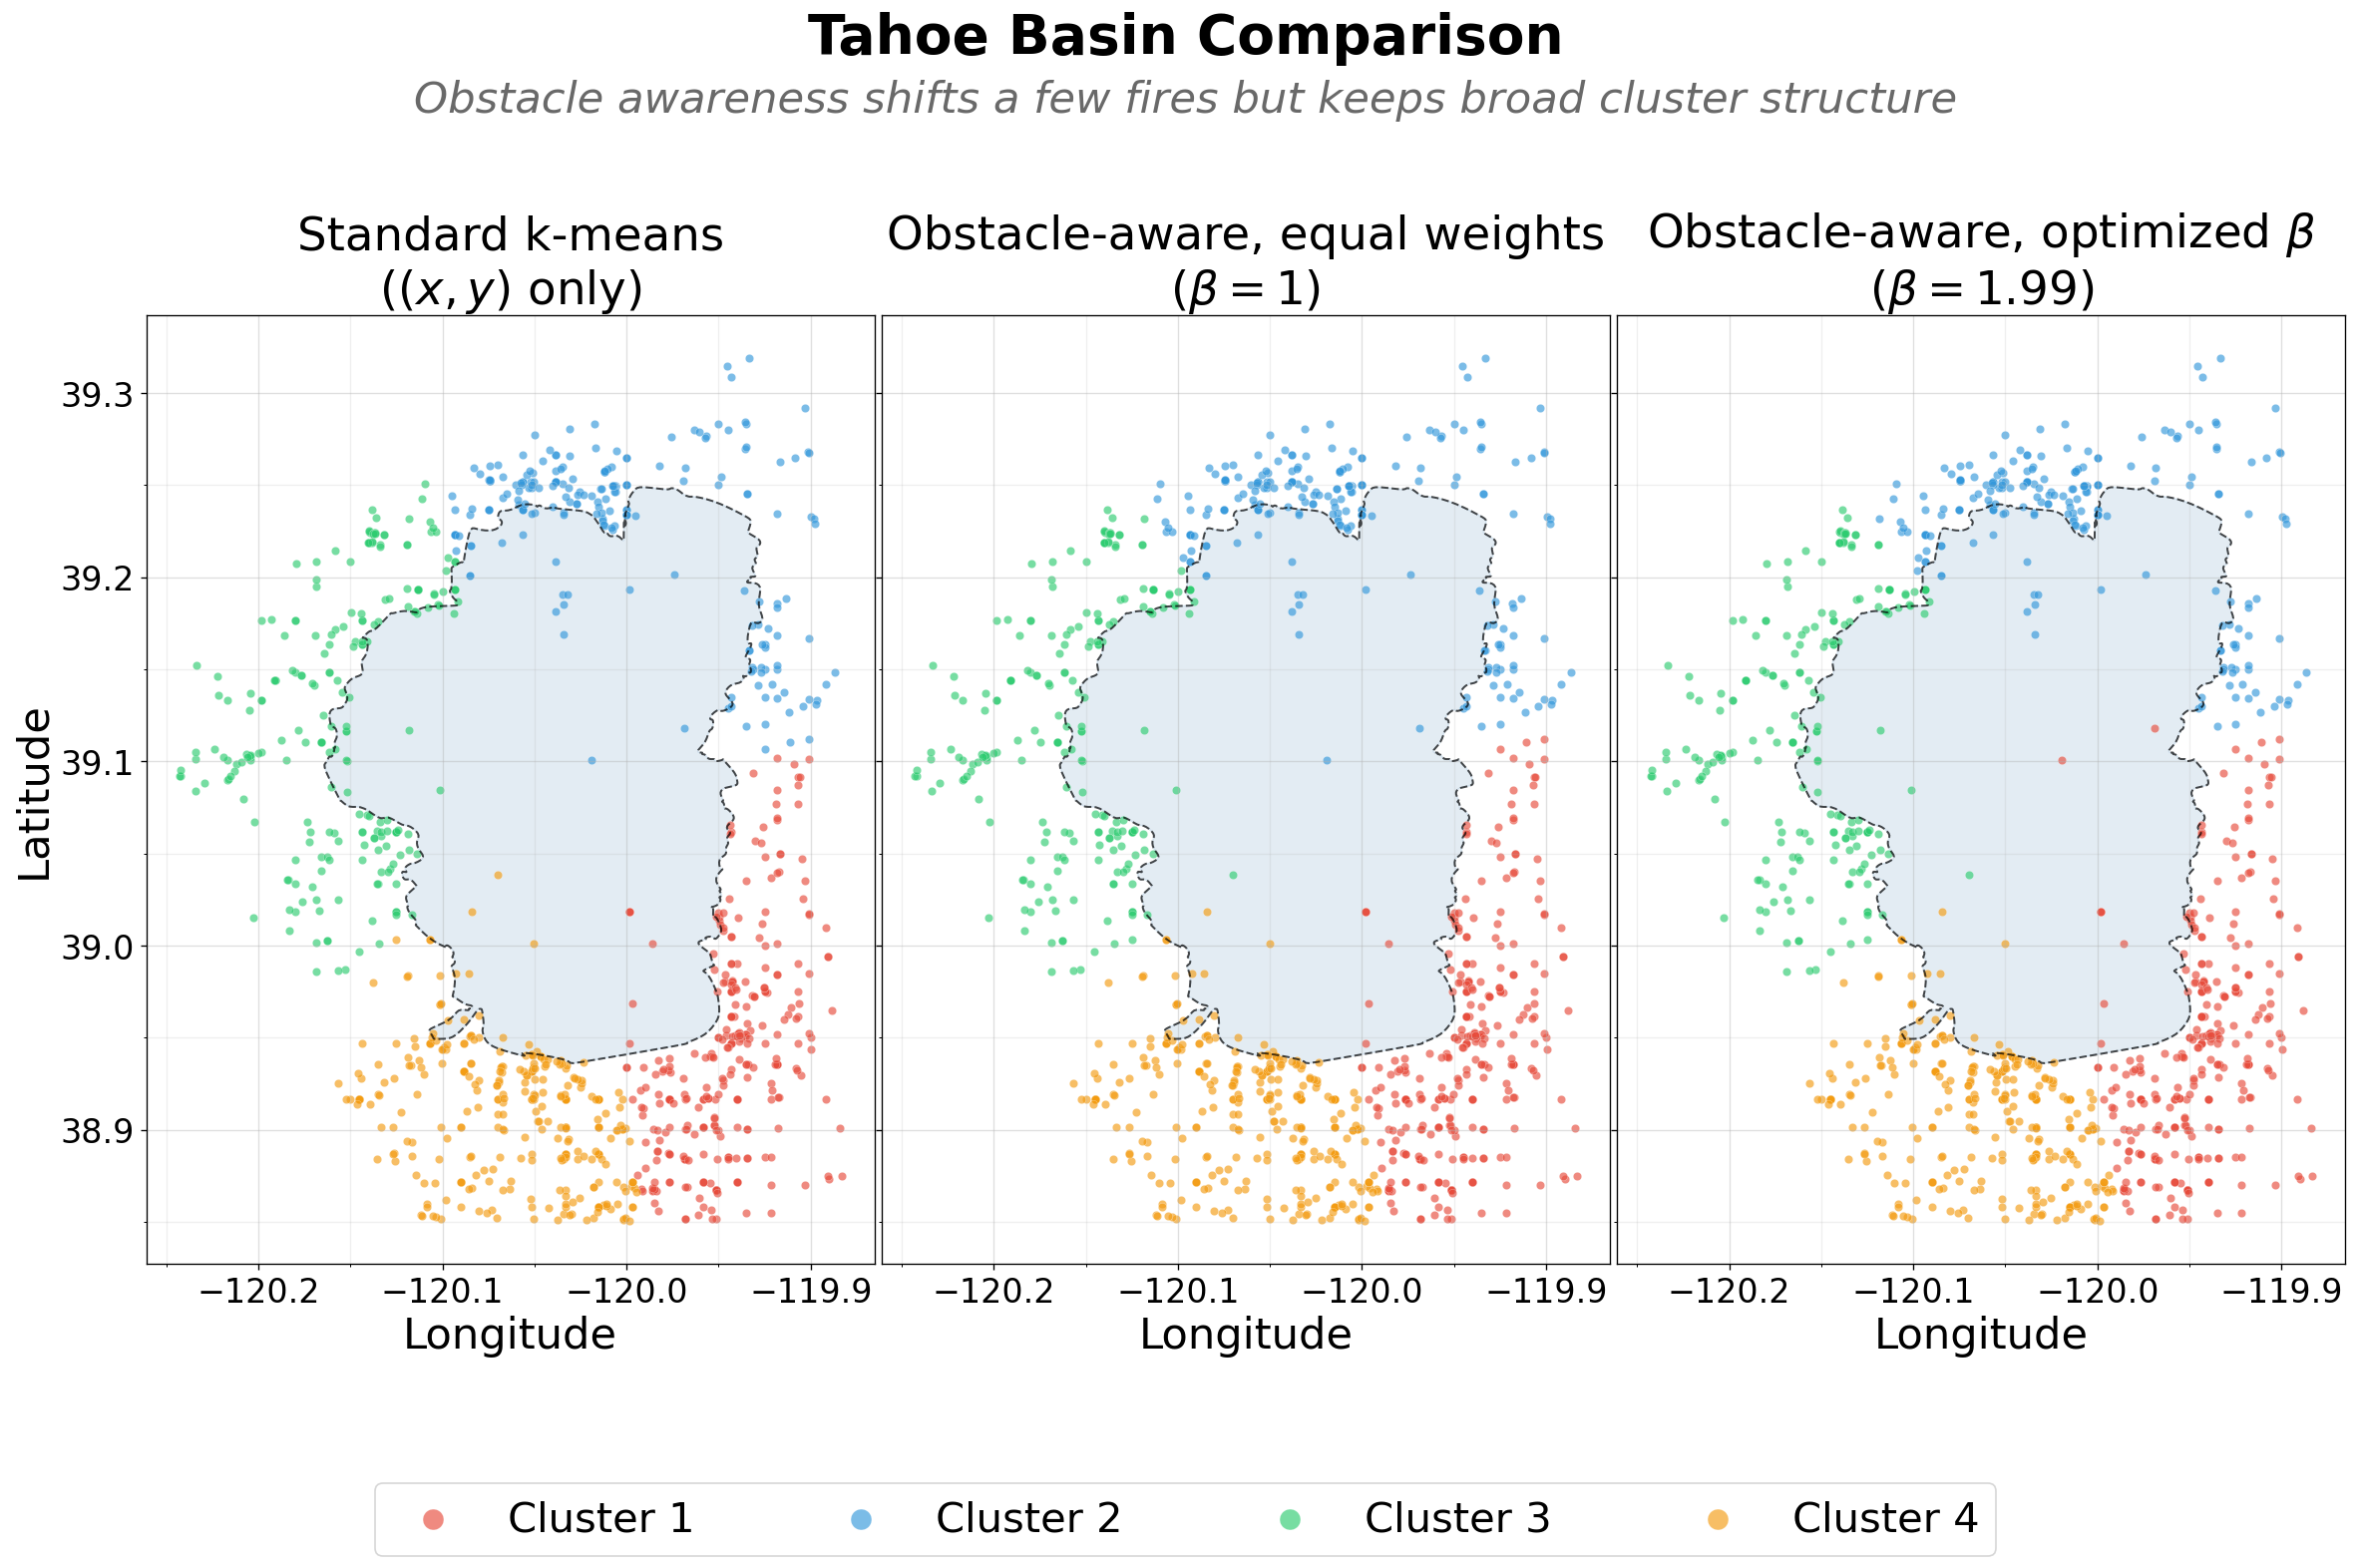
\includegraphics[width=1.1\textwidth]{figures/tahoe_basin_three_methods.png}}
\caption{Lake Tahoe basin: the same 1,068 fires clustered three ways. The four-way spatial split is stable across all panels; the obstacle parameter shifts a few fires near the borders between clusters but does not reorganize the clustering. From equal weights to the optimized $\beta$, the per-cluster spans rebalance: one cluster tightens sharply while another loosens, so the mean span improves only modestly even though individual clusters shift more.}
\label{fig:tahoe-basin-compare}
\end{figure}
 
At the basin scale, obstacle awareness gives a modest but real improvement: equal weights captures most of it (6.6\%), and tuning $\beta$ adds a little more (8.1\%).
 
\subsection{Near-shore scale: three methods}
\label{sec:tahoe-near}
 
The near-shore subset asks how the method behaves when fires are concentrated right next to the obstacle. For each fire, the straight-line distance to its projection on the shoreline is computed (with a degree-to-km conversion using $1^\circ$ latitude $\approx 111$ km and $1^\circ$ longitude $\approx 87$ km at this latitude). The subset is the 296 fires within 1 km of the shore, $27.7\%$ of the basin total.
 
The 1 km threshold is chosen to give a fraction of fires similar to Lake Mead's near-shore subset (which uses 5 km to keep $\approx 25\%$ of its fires).
 
\paragraph{Three methods on the subset.}
The same three clusterings run on the 296-fire subset. Standard k-means converges in 5 iterations with sizes 93, 71, 51, and 81 and a mean span of $0.2246$ (about 26.6 km). Equal weights converges in 9 iterations with sizes 94, 51, 71, 80 and a mean span of $0.2261$ -- slightly \emph{worse} than standard k-means by 0.6\%. The $\beta$ sweep selects $\beta = 0.86$, which sits in a wide stable low-$J$ region; refitting produces cluster sizes identical to standard k-means (93, 71, 51, 81) and a mean span of $0.2246$ (26.6 km), recovering standard k-means exactly.
 
Figure~\ref{fig:tahoe-near-compare} shows the three panels.
 
\begin{figure}[H]
\centering
\makebox[\textwidth]{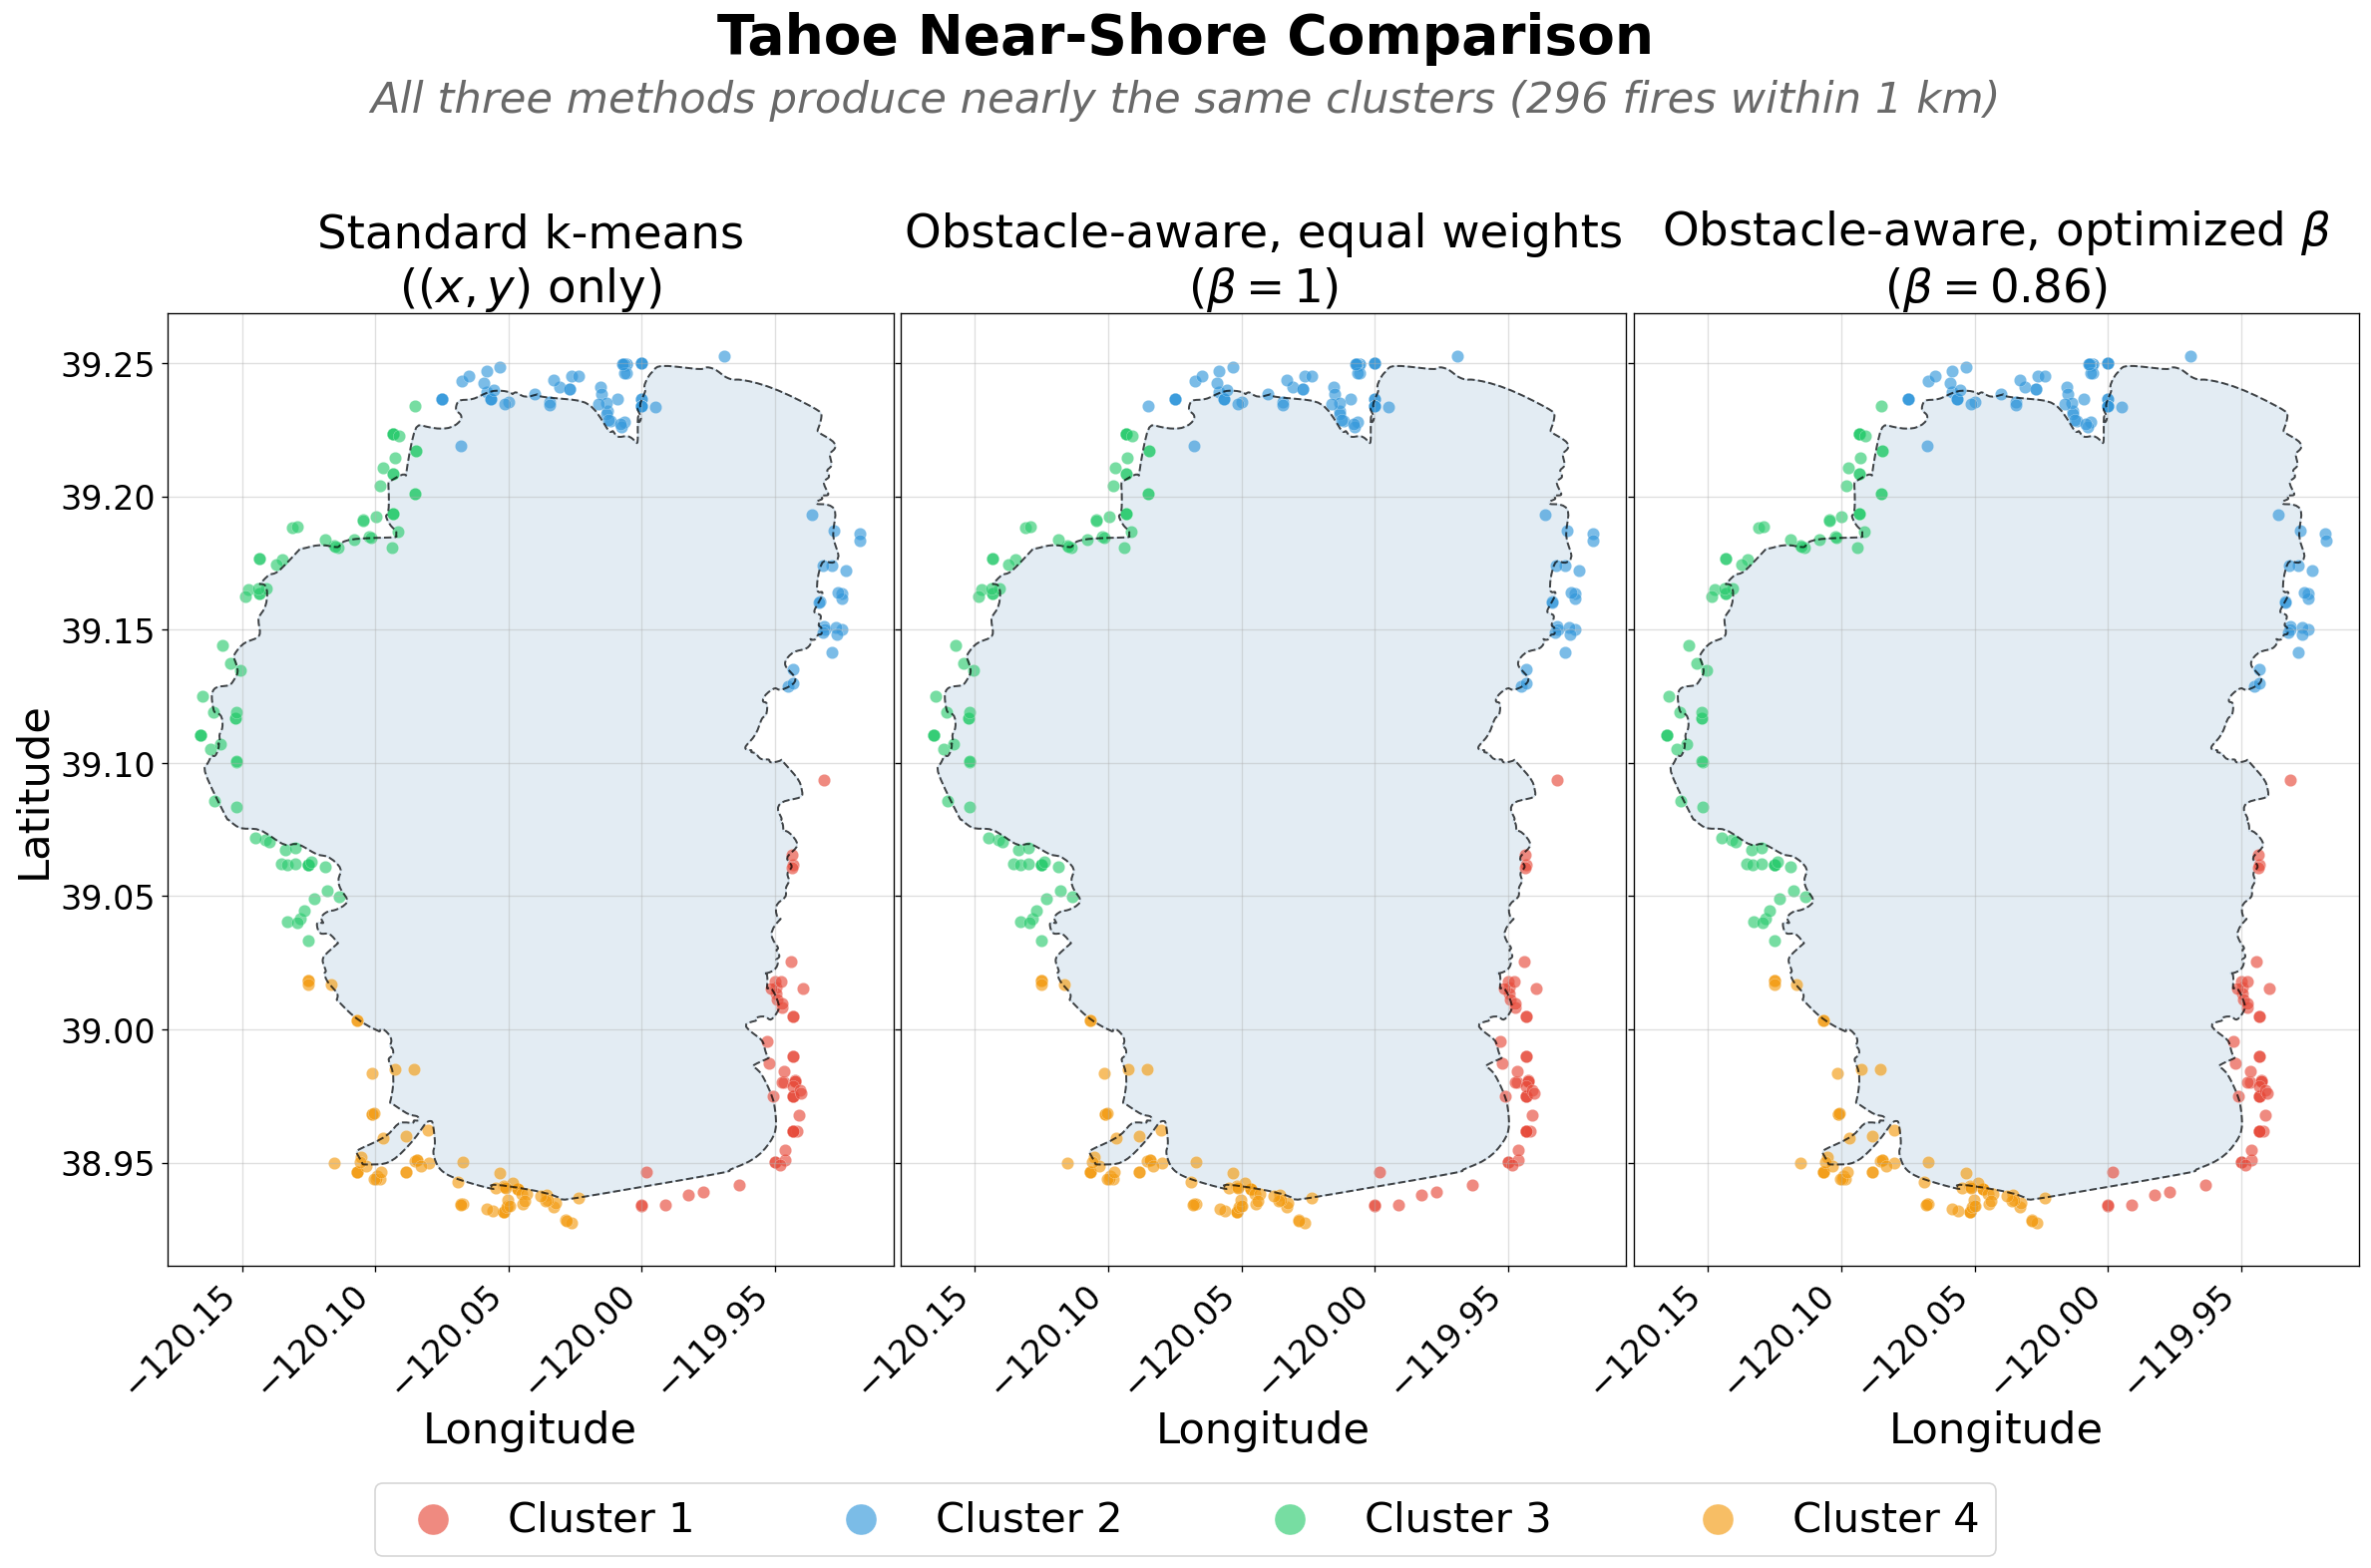
\includegraphics[width=1.2\textwidth]{figures/tahoe_near_three_methods.png}}
\caption{Lake Tahoe near-shore: the three clusterings are nearly indistinguishable. With fires already concentrated in a thin ring around the lake, the four clusters break the ring into four arcs the same way under all three methods. Standard k-means and the optimized obstacle-aware clustering produce identical per-cluster spans.}
\label{fig:tahoe-near-compare}
\end{figure}
 
The visual sameness across panels matches the numbers: it seems that near the shore, the obstacle parameter has nothing to add.
 
\subsection{Tahoe summary}
 
Across the two scales, Tahoe gives a clean but limited result. The obstacle parameter helps at the basin scale -- an $8.1\%$ improvement over standard k-means at the optimized $\beta$, tightening the average cluster's shoreline footprint from 31.3 km to 28.8 km, with equal weights already capturing most of that -- and helps not at all near the shore, where the optimized clustering recovers standard k-means exactly (26.6 km in both cases).
 
The pattern is the opposite of what one might guess. The arc-length parameter was built around the obstacle, so it is tempting to expect it to matter most right next to the obstacle. But near the shore, a fire's position around the lake is almost entirely determined by its $(x, y)$ coordinates: a thin ring of fires makes $s$ nearly redundant with the coordinates, so adding $s$ adds little new information. Across the full basin, fires sit at varying distances from the lake, and a distant fire's $(x, y)$ position does not pin down which stretch of shoreline it belongs to, so $s$ carries information the coordinates do not.
 
Now, we will switch our obstacle boundary to Lake Mead, whose multi-arm geometry tells a very different story near the shore.

%==============================================================
\section{Case Study: Lake Mead}
\label{sec:mead}
%==============================================================
Lake Mead's shape differs substantially from that of Lake Tahoe. Formed by Hoover Dam on the Colorado River, it is a long, narrow reservoir with several major arms, including the main eastern basin, the northern Overton Arm, the southwestern Boulder Basin, and a channel extending south toward the dam. Whereas Tahoe is roughly a single compact oval, Mead consists of a branching network of elongated inlets and basins. If the usefulness of the obstacle parameter depends on lake geometry, Lake Mead is where any contrast with Tahoe should appear.
 
\subsection{Data and boundary}
 
The fire records come from the same FPA FOD source~\cite{fpafod} as Tahoe. Without an official basin polygon for Mead, the query uses a bounding box of roughly $\pm 0.4^\circ$ in latitude and $\pm 0.65^\circ$ in longitude around the lake, capturing fires within roughly 20 km of any part of it. The SQL pull returned 1,059 fires (1992--2020). Dropping missing-cause records left 844 fires, the working dataset.
 
The shoreline comes from the USGS NHD~\cite{nhd}, in layer 12 (large-scale waterbodies). Querying that layer by name and unioning every feature above 1 sq km captures the lake's shape (548.5 sq km) and gives a faithful shoreline to project fires onto.
 
The unioned polygon has 74,403 vertices, much finer than the clustering needs. Simplifying with Douglas-Peucker at a tolerance of about 450 m brings the vertex count down to 418 while preserving the major arms. A cubic spline fit through those vertices gives the closed boundary curve $\gamma(t)$. The resulting perimeter is 686.2 km -- nearly six times Tahoe's 118.3 km, reflecting the complex multi-arm shoreline.
 
\subsection{Projecting fires onto the shoreline}
 
Each of the 844 fires is projected onto the boundary spline, yielding its arc-length position $s \in [0,1]$. The values cover the full range, $0.011$ to $0.988$, so fires touch every stretch of shoreline.
 
\begin{figure}[H]
\centering
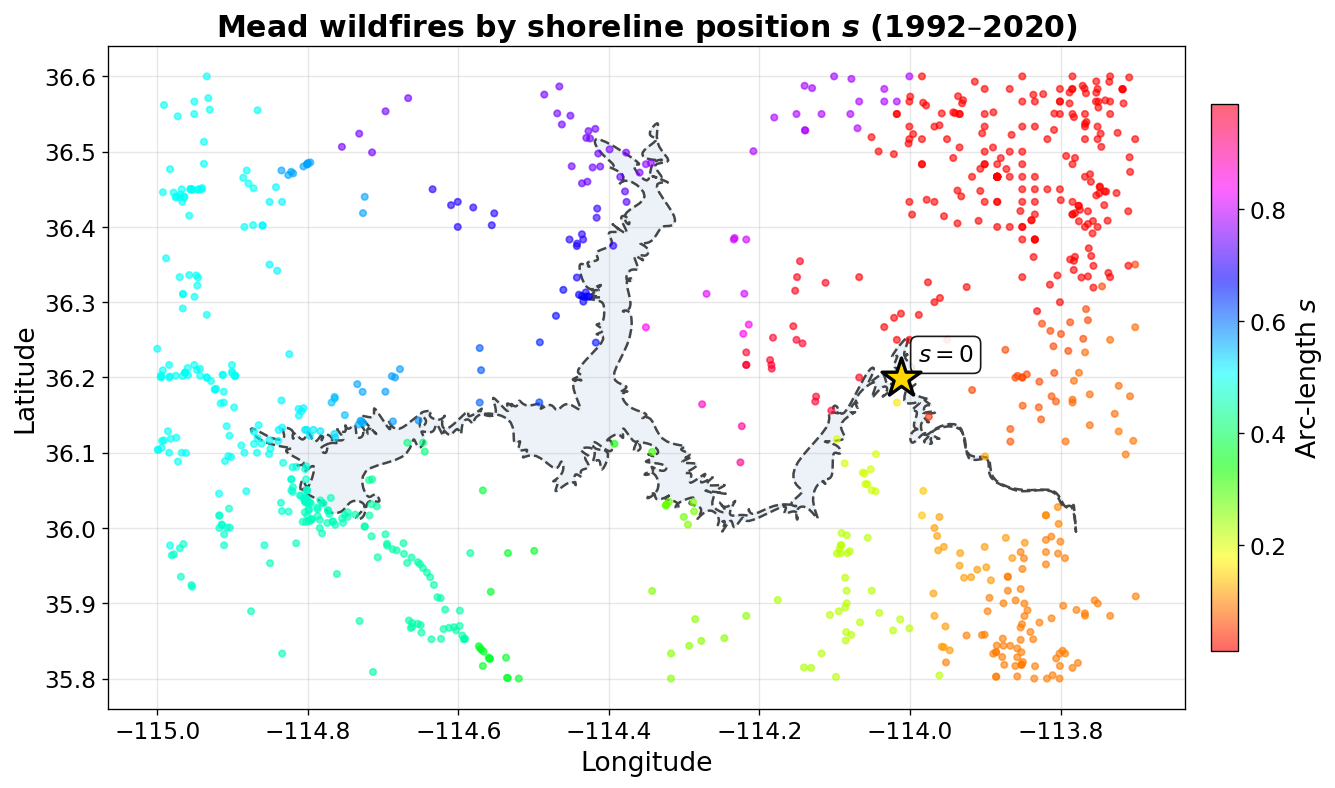
\includegraphics[width=\textwidth]{figures/mead_fires_by_s.png}
\caption{Lake Mead wildfires (1992--2020) colored by arc-length position $s$ along the shoreline. The HSV colormap wraps from red back to red across the seam at $s = 0$. The multi-arm geometry is visible in the color bands, which trace down each arm in turn as $s$ moves around the loop.}
\label{fig:mead-s}
\end{figure}
 
\subsection{Basin scale: three methods}
\label{sec:mead-basin}
 
The three clusterings run on all 844 fires, with the same setup as Tahoe.
 
\paragraph{Standard k-means (baseline).}
Standard k-means on scaled $(x, y)$ converges in 7 iterations and produces four clusters with sizes 185, 124, 273, and 262 fires. The mean arc-length span is $0.3412$, or about 234.1 km of shoreline per cluster on average. That number is much larger than Tahoe's 31 km -- not because Mead's clusters are looser as a fraction of the loop (Tahoe's was $0.265$ vs Mead's $0.341$), but because the loop itself is so much longer. Each Mead cluster covers about a third of a 690 km shoreline.
 
\paragraph{Obstacle-aware at equal weights.}
Adding $s$ as a clustering feature with $\beta = 1$ produces a clustering identical to standard k-means: the per-cluster spans are exactly the same, and the mean span comes out at $0.3412$ (234.1 km), a $0.0\%$ change. At this weighting the shoreline term is not strong enough to push any fires across cluster boundaries on Mead's basin-scale data; the clustering reorganizes only once $\beta$ is tuned higher.
 
\paragraph{Obstacle-aware at optimized $\beta$.}
The $\beta$ sweep runs the same 30-point grid from $\beta = 0.05$ to $\beta = 2.0$. Figure~\ref{fig:mead-basin-sweep} shows $J$ and span across the grid.
 
\begin{figure}[H]
\centering
\makebox[\textwidth]{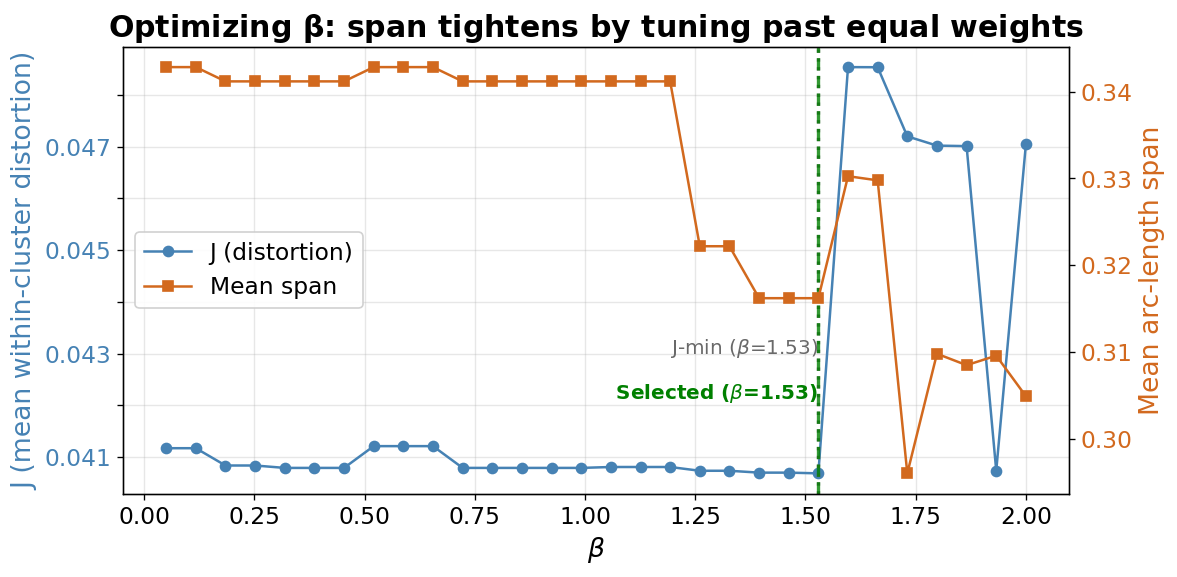
\includegraphics[width=1\textwidth]{figures/mead_basin_beta_sweep.png}}
\caption{Mead basin: $J$ and mean span across the $\beta$ grid. $J$ is nearly flat across a wide stretch, and within that region the span is flat too. The selection lands at $\beta = 1.53$, the lowest-$J$ point in the stable region; a marginally lower span past the region sits at an isolated low-$J$ point surrounded by higher-$J$ neighbors, and the stability filter excludes it.}
\label{fig:mead-basin-sweep}
\end{figure}
 
The selection picks $\beta = 1.53$. The grid minimum is also at $\beta = 1.53$, and $J$ is flat enough nearby that the stability filter is easily satisfied. Refitting at this $\beta$ gives cluster sizes 276, 183, 124, and 261, and a mean span of $0.3162$ (about 217.0 km). That is a $7.3\%$ improvement over standard k-means, tightening the average cluster's shoreline footprint from 234.1 km to 217.0 km -- a 17 km tightening.
 
\paragraph{Comparison.}
Figure~\ref{fig:mead-basin-compare} shows the three clusterings.
 
 
 
\begin{figure}[H]
\centering
\makebox[\textwidth]{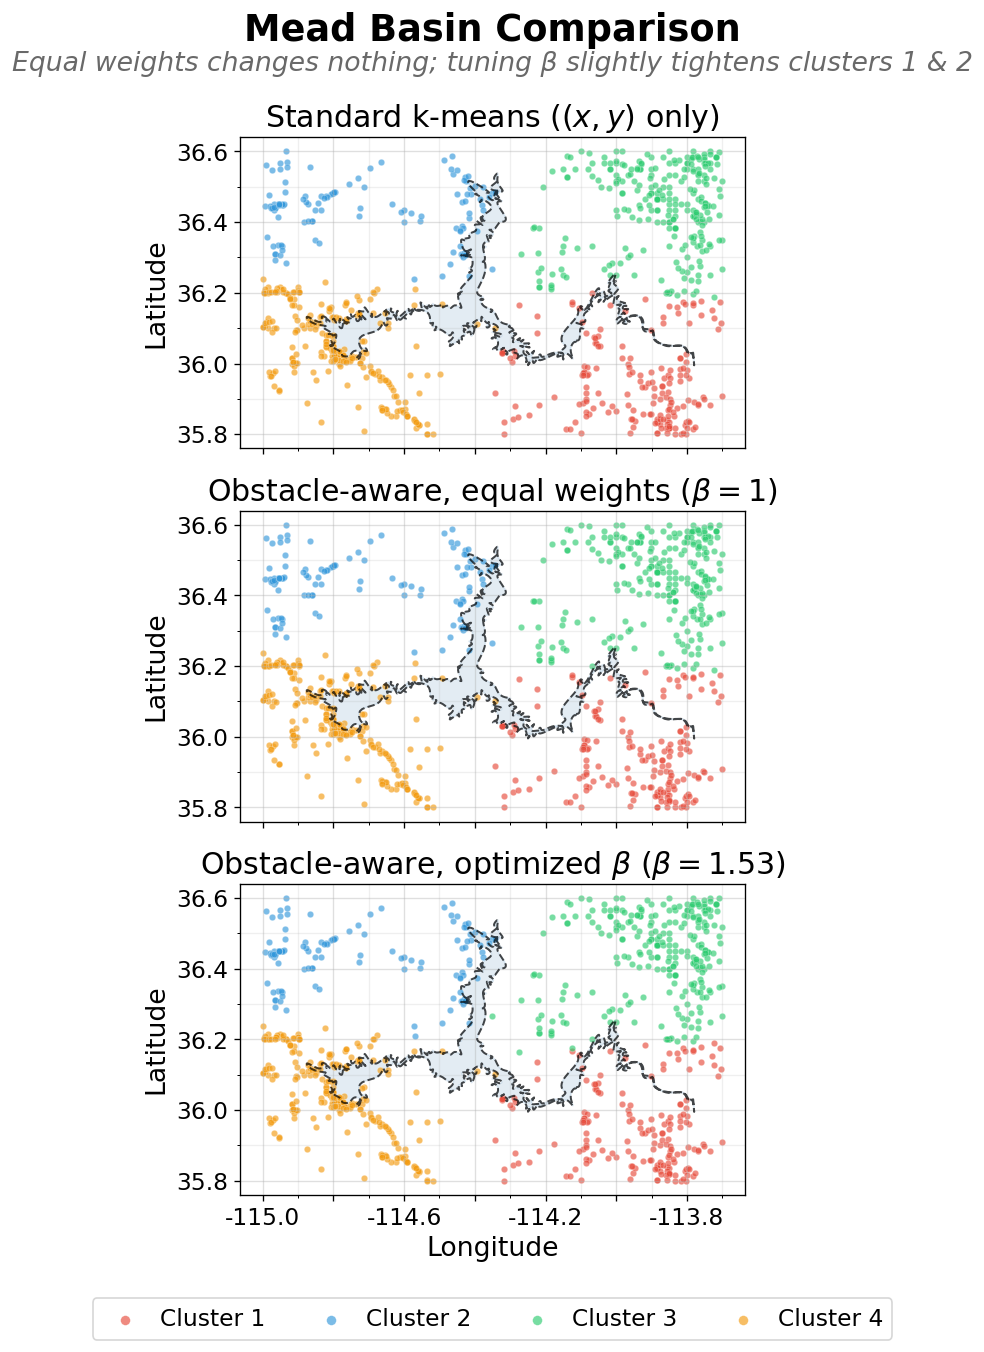
\includegraphics[width=0.8\textwidth]{figures/mead_basin_three_methods.png}}
\caption{Lake Mead basin: the same 844 fires clustered three ways, with colors aligned across panels. The four-way layout is stable in all three panels (one cluster per region of the basin), and standard k-means and equal weights produce essentially identical clusterings. The optimized $\beta$ shifts boundaries slightly along the lake's arms, particularly around the central body and the southeastern arm where some fires move between clusters.}
\label{fig:mead-basin-compare}
\end{figure}
 
At the basin scale, the improvement is concentrated in one cluster. Looking across the three methods, the per-cluster spans of Clusters 1, 3, and 4 stay close to their standard k-means values (Cluster 1: $0.397 \to 0.373$, Cluster 3: $0.305 \to 0.305$, Cluster 4: $0.322 \to 0.322$). Cluster 2 is where the obstacle parameter does its work, tightening from $0.341$ to $0.266$. So the basin-scale improvement is not a broad retightening across all four clusters; it is one cluster getting much tighter while the others barely move.
 
\subsection{Near-shore scale: three methods}
\label{sec:mead-near}
 
The near-shore subset uses a 5 km threshold, chosen to keep about $25\%$ of the basin's fires ($214$ fires, $25.4\%$). This is close to Tahoe's $27.7\%$ near-shore share so the two near-shore comparisons are on comparable footing in terms of data volume.
 
\paragraph{Three methods on the subset.}
Standard k-means converges in 3 iterations with very uneven cluster sizes -- 126, 16, 40, and 32 fires -- and a mean span of $0.2425$ (about 166.4 km).
 
Equal weights converges in 8 iterations with sizes 33, 126, 40, and 15, and a mean span of $0.2204$ (151.2 km). That is a $9.1\%$ improvement over standard k-means -- already substantial, and much better than Tahoe's near-shore equal-weights result, which actually made things slightly worse.
 
The $\beta$ sweep shows where the obstacle-aware version finds further room to tighten (Figure~\ref{fig:mead-near-sweep}).
 
\begin{figure}[H]
\centering
\makebox[\textwidth]{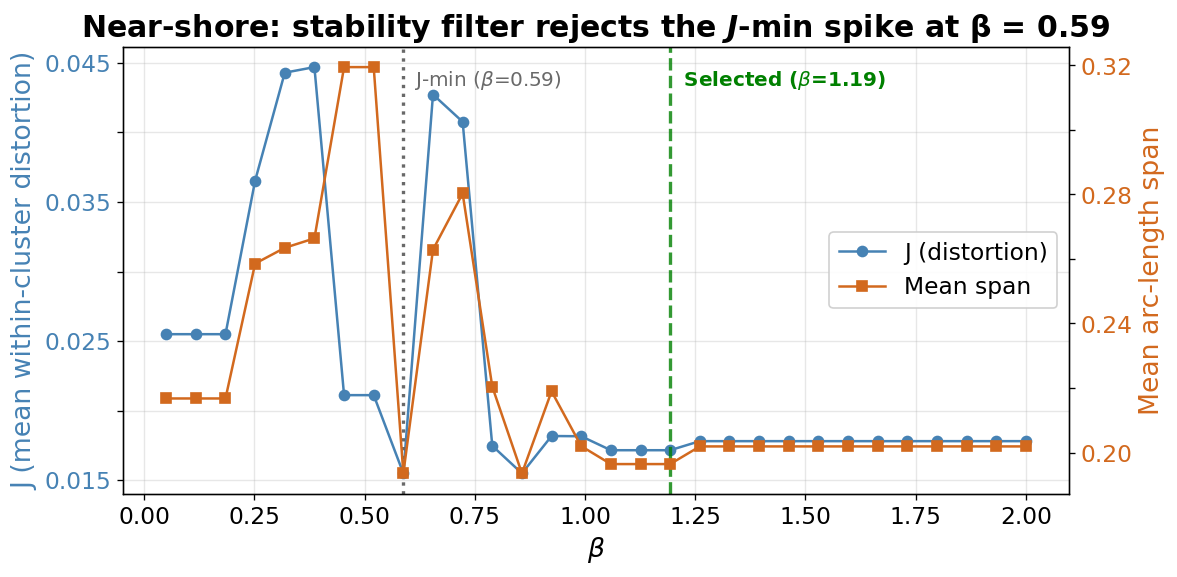
\includegraphics[width=1\textwidth]{figures/mead_near_beta_sweep.png}}
\caption{Mead near-shore: $J$ and mean span across the $\beta$ grid. The grid minimum sits at $\beta = 0.59$, where $J$ drops to a sharp point surrounded by much higher-$J$ neighbors. The stability filter rejects this isolated dip. The selection lands at $\beta = 1.19$, where $J$ and span are both stable and every cluster contains more than 10 fires.}
\label{fig:mead-near-sweep}
\end{figure}
 
The selection works through both filters here. The lowest-$J$ point on the grid is $\beta = 0.59$, but $J$ at that $\beta$ is an isolated spike: the neighbors on either side jump to much higher $J$, so the clustering at $\beta = 0.59$ only holds at that exact weighting. The lowest-span solutions in that low-$\beta$ region also have a cluster collapsed to a handful of fires (under the 10-fire floor), so the cluster-size constraint applies as well. Both filters point toward the stable region past $\beta \approx 1.0$, where the selection lands at $\beta = 1.19$.
 
Refitting at $\beta = 1.19$ gives cluster sizes 34, 126, 14, and 40, and a mean span of $0.1964$ (about 134.8 km). That is a $19.0\%$ improvement over standard k-means, the largest gain of any case in the project.
 
\paragraph{Comparison.}
Figure~\ref{fig:mead-near-compare} shows the three clusterings.
 
\begin{figure}[H]
\centering
\makebox[\textwidth]{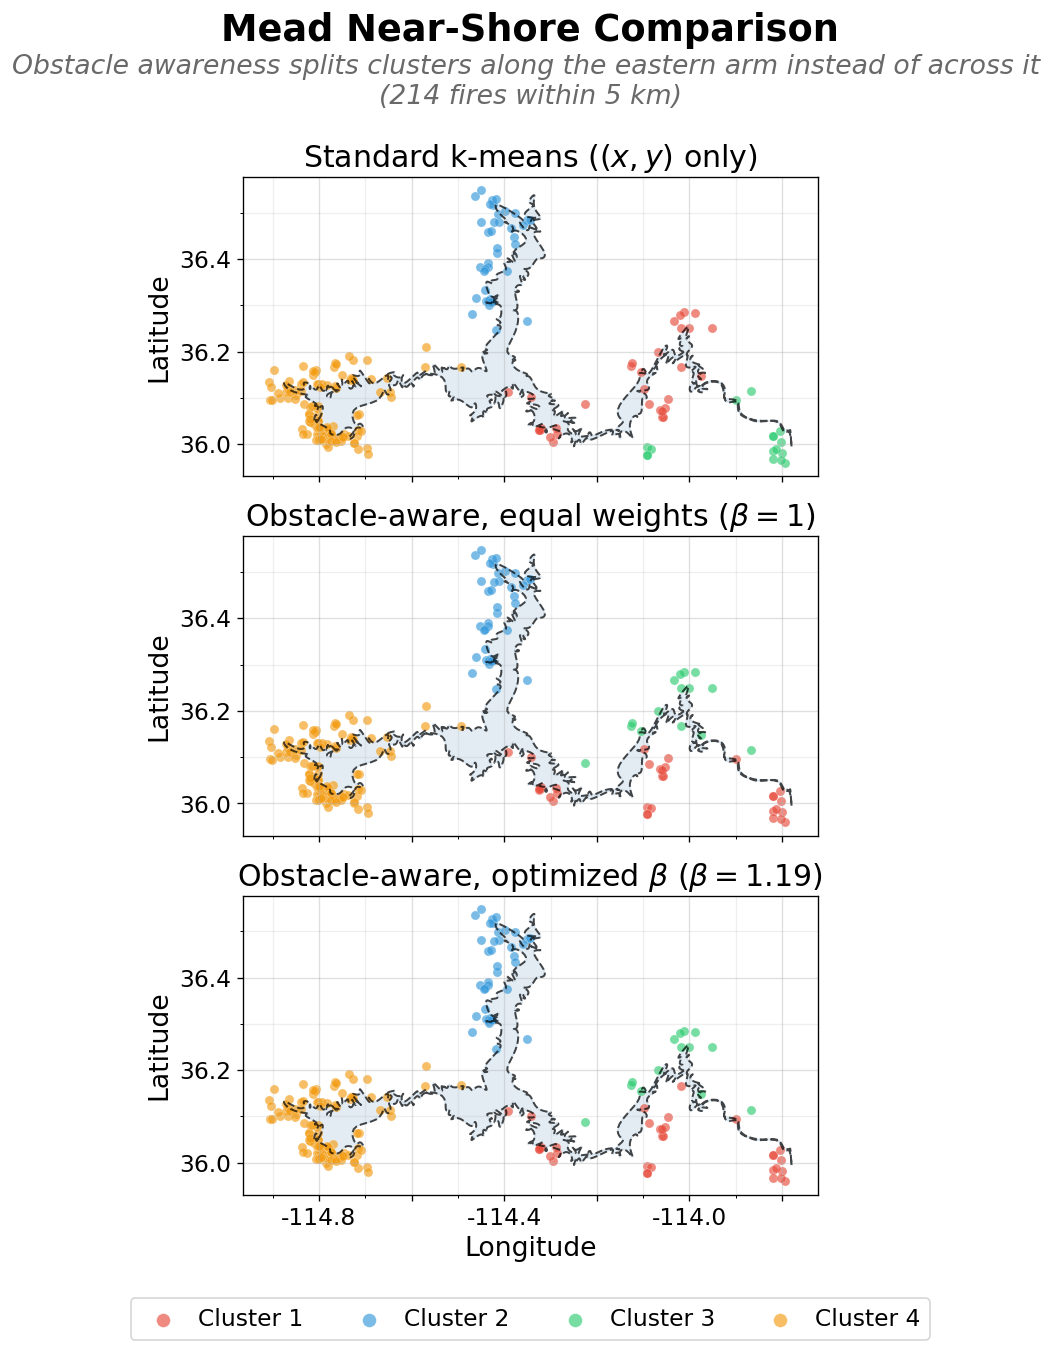
\includegraphics[width=.8\textwidth]{figures/mead_near_three_methods.png}}
\caption{Lake Mead near-shore: the standard k-means clustering (left) splits the data unevenly, with the green cluster reaching across the water rather than following one stretch of shore. Both obstacle-aware versions pull the green cluster onto a single arm, splitting the eastern shoreline cleanly between the northeastern (green) and southeastern (red) arms. The improvement comes almost entirely from the green cluster, which tightens from a span of $0.42$ under standard k-means to about $0.24$ under both obstacle-aware variants.}
\label{fig:mead-near-compare}
\end{figure}
 
The mechanism is visible in the figure. Under standard k-means, Clusters 1 and 3 overlap across the eastern arm. Although the north and south shorelines of this arm are close in straight-line distance, they are much farther apart when measured by arc-length distance. The optimized obstacle algorithm accounts for this difference and shifts assignments so that Clusters 1 and 3 are almost completely separated, lying below and above the arm, respectively. All fires in Cluster 3 lie on the arm's north shoreline and all but one of Cluster 1's fires lie on the south shoreline. This improvement is most reflected in the arc-length span of Cluster 1: $0.420 \to 0.236 \to 0.236$ across the three methods. The other three clusters barely move ($0.186, 0.157, 0.206$ under standard k-means, nearly identical under the obstacle-aware versions). So the near-shore $19\%$ gain is not a broad retightening; it is the shoreline parameter fixing a cluster that standard k-means stretches across the water.
 
\subsection{Mead summary}
 
Mead behaves very differently from Tahoe. At the basin scale, both lakes show similar percent improvements at the optimized $\beta$ ($7.3\%$ for Mead, $8.1\%$ for Tahoe), although the absolute km tightening is much larger on Mead ($17$ km vs $2.5$ km) because the shoreline is six times longer. The substantive difference shows up near the shore: where Tahoe's optimized near-shore clustering recovers standard k-means exactly ($0.0\%$ improvement), Mead's reaches $19.0\%$, the project's largest gain. In absolute terms, Mead's near-shore clusters tighten by about 32 km on average. The figure makes the mechanism plain -- standard k-means mixes two clusters across an arm of the lake,  and the arc-length parameter pulls them onto separate sides. 

%==============================================================
\section{Cross-Lake Comparison}
\label{sec:cross-lake}
%==============================================================
 
Running the same method on Tahoe and Mead, with the same $k$ and the same selection procedure, lets us see whether the obstacle parameter behaves the same way on lakes of contrasting shape.
 
\subsection{Side-by-side results}
 
Table~\ref{tab:cross-lake} lists the headline numbers for all four lake / scale combinations. Each row reports the number of fires, the mean shoreline span under standard k-means and under the optimized obstacle-aware clustering (in km), and the percent improvement.
 
\begin{table}[H]
\centering
\caption{Cross-lake comparison: span improvement from obstacle-aware clustering. The standard and optimized columns give the mean shoreline span per cluster in km, computed as the dimensionless span times the lake's total perimeter (118.3 km for Tahoe, 686.2 km for Mead). The improvement column is the percent reduction in span vs standard k-means at the same scale.}
\label{tab:cross-lake}
\rowcolors{2}{gray!8}{white}
\begin{tabular}{llrrrr}
\toprule
Lake & Scale & Fires & Standard span (km) & Optimized span (km) & Improvement \\
\midrule
\multirow{-1}{*}{Tahoe}
  & Basin      & 1{,}068 & 31.3  & 28.8  & $+8.1\%$  \\
  & Near-shore &   296   & 26.6  & 26.6  & $\phantom{+}0.0\%$ \\
\midrule
\multirow{-1}{*}{Mead}
  & Basin      &   844   & 234.1 & 217.0 & $+7.3\%$  \\
  & Near-shore &   214   & 166.4 & 134.8 & $+19.0\%$ \\
\bottomrule
\end{tabular}
\end{table}
 
Two patterns stand out. At the basin scale, both lakes improve by similar percentages ($8.1\%$ for Tahoe, $7.3\%$ for Mead).  At the near-shore scale, the two lakes diverge: Tahoe has no change, Mead has the project's largest improvement at $19.0\%$. 
 
\subsection{Why geometry matters}
 
The pattern in Table~\ref{tab:cross-lake} points to one potential explanation. The arc-length parameter $s$ helps when it carries information the $(x, y)$ coordinates do not. On a compact, roughly oval lake like Tahoe, this almost never happens: a fire's position around the shoreline is closely determined by its planar coordinates, so $s$ is largely redundant. On a long, multi-arm lake, two fires can sit close in straight-line distance while being far apart along the shore, because the shore runs out to the tip of one arm and back before reaching the other. There $s$ encodes something the coordinates cannot.
 
The Mead near-shore figure in Section~\ref{sec:mead-near} makes this visible: standard k-means mixes two clusters across the water and the arc-length parameter splits them onto their own shoreline. Tahoe has no separate, thin arms for a cluster to bridge across, so $s$ has no analogous opportunity to help.  The two lakes suggest that obstacle-aware k-means tightens clusters when the lake's shape makes shoreline distance diverge from straight-line distance. Compact shapes barely diverge between the two, so the gains are small. Multi-arm shapes diverge sharply, particularly near the shore, so the gains are largest exactly where the geometry is most distorted by the obstacle. Confirming this pattern would require running the method on more lakes spanning a range of shapes (see Section~\ref{sec:more-lakes}).
 
\subsection{One potential confound}
 
The cross-lake comparison is not a completely controlled experiment. The two near-shore subsets were chosen to keep a similar fraction of each lake's fires -- about a quarter, $27.7\%$ for Tahoe and $25.4\%$ for Mead -- rather than to use the same absolute distance threshold. The chosen thresholds were 1 km for Tahoe and 5 km for Mead.
 
Matching by fraction keeps the two subsets comparable in terms of how much data each carries, but it leaves a difference in how close to shore each subset's fires actually are. Mead's near-shore fires sit on average farther from the water than Tahoe's. Some portion of the difference between $0\%$ improvement (Tahoe near-shore) and $19\%$ (Mead near-shore) could plausibly come from this distance difference rather than from lake shape.
 
The geometric mechanism is likely responsible for at least part of the $19\%$ improvement, although additional experiments would be needed to disentangle the effects of lake geometry from those of fire distance (see Section~\ref{sec:more-lakes}).

%==============================================================
\section{Attribute Analysis}
\label{sec:attributes}
%==============================================================
 
So far the analysis has used only location. Each fire data vector contained only its $(x, y)$ coordinates and arc-length position $s$. However, as McMahon et al.~\cite{mcmahon2022} show, it can be useful to consider how clusters differ in behavioral attributes too. Those authors built attributes into the clustering distance directly, with a tunable weight setting how much the attributes pull against geography, and used a separate set of held-back attributes to score the resulting clusters. We do something much lighter here: rather than tuning the clustering to enforce attribute differences, we cluster on location only and check, after the fact, whether the location-based clusters happen to differ in behavior. 

Two attributes were carried alongside the spatial features: total fire size in acres (log-transformed) and cause, binary-encoded as natural or human-caused. For each clustering, we tested cluster differences in these attributes using the Kruskal-Wallis test with Dunn's follow-up and a Bonferroni correction, reporting the fraction of the six possible cluster pairs that differ significantly per attribute. The choice of Kruskal-Wallis followed by Dunn's was influenced by McMahon et al.~\cite{mcmahon2022}, who used the same pair of tests (alongside ANOVA and Tukey, where parametric assumptions held) to measure attribute separation between clusters. We use the non-parametric option throughout because fire size is heavily right-skewed. For each lake, we ran the test at the scale where the obstacle parameter made the most improvement on clustering: the basin for Tahoe ($+8.1\%$ improvement) and the near-shore for Mead ($+19\%$). 
 
On the Tahoe basin, the four clusters show almost no attribute separation. Under standard k-means, $0$ of $6$ cluster pairs differ in fire size and $1$ of $6$ differ in cause; the overall significant fraction is $0.08$. The optimized clustering gives an identical $0.08$. Tahoe's basin is geographically small with a relatively homogeneous fire environment, so the location-based clusters do not pick up systematic differences in fire behavior. 
 
The Mead near-shore tells a different story. Under standard k-means, $3$ of $6$ pairs differ in fire size and $3$ of $6$ in cause, an overall fraction of $0.50$. Since the clustering only used location, this means fire behavior around Mead's shore is not spread evenly -- some stretches see larger fires, or more human-caused ones, than others. The optimized obstacle-aware clustering shows slightly \emph{less} attribute separation, not more: $3/6$ pairs still differ in fire size, but only $1/6$ in cause, dropping the overall fraction to $0.33$. Tightening clusters along the shoreline cut a little across the attribute patterns, but the fires that moved between clusters carried slightly different attribute distributions with them. The obstacle-aware method is better at what it optimizes (span) and slightly worse at a metric it did not see during fitting (attribute distinctness). 
 
A natural extension would address the cohesion-distinctness tradeoff directly.  Our composite distance \eqref{eq:composite} already includes an optional $\gamma$ term for attributes (held at zero throughout this report), and the $\beta$-selection procedure could be extended to a two-dimensional $(\beta, \gamma)$ grid with an objective combining span tightness and attribute separation. That would let the user pick where on the cohesion-distinctness tradeoff to land for any given application.

%==============================================================
\section{Discussion}
\label{sec:discussion}
%==============================================================

\subsection{Why this matters for wildfires}

The introduction described wildfires as point data with real safety and resource-allocation stakes -- response stations should sit central to where fires actually occur, in terms of how a vehicle would have to travel rather than straight-line distance. The lake comparisons here speak to that: when a lake's shape makes the shore meaningfully different from a straight line, the obstacle-aware clusters line up with the shore better than standard k-means clusters do, which is closer to the way response would actually have to move around the water.

The results don't say where to actually put stations. A real placement study would need to know how response works on a particular lake -- by road, water, or air -- along with existing infrastructure and historical response times. The clustering gives a more grounded starting point than standard k-means when the lake's shape calls for it, and the next step would be testing the cluster centroids against real operational data.

\subsection{More lakes}
\label{sec:more-lakes}

Tahoe and Mead were deliberately chosen as lakes with contrasting shapes -- compact oval against branching reservoir -- and their near-shore results line up with the geometric mechanism described in Section~\ref{sec:cross-lake}. But $n = 2$ is too small a sample for a general claim about how lake shape governs the obstacle parameter's value. Confirming the pattern would need more lakes, ideally chosen to span a real range of shapes (compact ovals, single-arm lakes, multi-arm reservoirs, branching lakes with many small fingers) so that shape becomes something we can vary on purpose rather than a contrast between two cases. With ten or twenty such lakes, the relationship between geometric complexity and the obstacle parameter's value could be characterized properly -- for instance, by testing a shape-complexity statistic (something like the ratio of perimeter to convex-hull perimeter) against the obstacle parameter's improvement.

The two near-shore subsets keep about a quarter of each lake's fires by using a 1 km threshold for Tahoe and 5 km for Mead. Holding the fraction constant keeps the two subsets comparable in data volume, but the threshold difference means Mead's near-shore fires sit on average farther from the water than Tahoe's. This confound cannot be cleanly separated with only two lakes. The natural fix is to sweep the threshold systematically on each lake -- across, say, 0.5 km to 10 km -- and watch how the improvement changes with distance. The distance effect would show up within each lake's curve, and the shape effect would show up as the difference between curves.
 
\subsection{Method refinements}
\label{sec:method-refine}
 
A few details of how the method was set up here could be spots for refinement in a future version.

The number of clusters was held at $k = 4$ across both lakes for a controlled comparison, driven by Tahoe's elbow plot. In practice, you would pick the best $k$ for each lake separately, and how the obstacle parameter behaves at other $k$ values -- particularly on lakes where the natural number of clusters differs from four -- is open.

The Mead near-shore clusters are small and uneven, with three of the four holding between 14 and 40 fires. This limits the statistical power of the attribute tests in Section~\ref{sec:attributes} and also limits how useful the clusters would be in practice, since a real fire station network would likely want roughly even coverage rather than a handful of stations handling most of the fires. The existing size floor only rules out truly degenerate clusters; an extension that targets evenness directly -- a balance penalty in the objective, or a balanced-k-means variant -- would be needed to fix this.

Boundary processing involves choices that were not systematically varied: the Douglas-Peucker simplification tolerance, the choice of cubic spline over alternative smooth curves, and lake-specific edits to the raw boundary polygon all matter for projection and span. Each was justified case-by-case rather than tested across alternatives.

Finally, the clustering used only location. As sketched in Section~\ref{sec:attributes}, including attributes would let the method trade between shoreline cohesion and attribute distinctness. The composite distance \eqref{eq:composite} already accommodates a third weighted term ($\gamma$, held at zero throughout); extending the $\beta$-selection procedure to a two-dimensional $(\beta, \gamma)$ grid with a combined objective is a direct generalization of what was done here.
 
\subsection{Other obstacles}
\label{sec:other-obstacles}
 
The method extends beyond lakes. The arc-length parameter $s$ requires a closed boundary curve, but other physical features could play the obstacle role: an island shoreline (where the obstacle is the inside of the curve rather than the outside), or a coastline segment treated as a non-closed curve with $s \in [0, 1]$ running end to end rather than wrapping. The composite distance and centroid update would carry over with some minor modifications. More broadly, the framework of adding a tuned non-Euclidean component to k-means distance applies anywhere a geographic feature distorts how points should be grouped, including mountain passes, highway networks, and administrative boundaries, though each context would need its own version of the projection step that gave fires their $s$ values here.
 


%==============================================================
\section{Conclusion}
%==============================================================

This report developed an obstacle-aware version of k-means and applied it to wildfire data around two lakes of contrasting shape. The method adds a single feature -- the normalized arc-length position $s$ of each fire along the shoreline -- to the standard $(x, y)$ feature vector, weighting $s$ against straight-line distance through one tunable parameter $\beta$. Setting $\beta = 0$ recovers standard k-means, so the method is a strict generalization. Tune $\beta$ by sweeping a grid and selecting among stable low-objective values by smallest mean shoreline span.

The two lakes tell a clear two-part story. At the basin scale, Tahoe and Mead behave similarly, both improving by roughly $7$-$8\%$ over standard k-means. At the near-shore scale they diverge: Tahoe's optimized clustering recovers standard k-means exactly, while Mead's gives the project's largest gain at $19\%$. The mechanism is visible in the figures. Mead's multi-arm geometry creates situations where two fires can sit close in straight-line distance but on opposite sides of a long, thin arm; reaching one from the other along the shore means going out to the arm's tip and back. The arc-length parameter registers that distance, and separates them into different clusters. Tahoe's compact oval has no separate arms for a cluster to bridge across, so $s$ carries no information the coordinates do not. The obstacle parameter helps to the extent that a lake's shape makes shoreline distance differ from straight-line distance.

The Mead near-shore clusters also carry some real attribute structure, which the obstacle-aware clustering slightly weakens as it tightens shoreline cohesion. This tradeoff points to an extension of the method: treating attributes as a third weighted term in the clustering distance. The cross-lake contrast rests on two lakes chosen for their shapes, so generalizing the geometric pattern would need more lakes and a threshold-sweep design to separate shape effects from absolute-distance effects.

%==============================================================
\section*{Acknowledgements}
%==============================================================

Many thanks to my master's advisor at North Carolina State University, Dr. Mansoor Haider, who suggested the idea of a tailored k-means algorithm with obstacle awareness and guided the development of the method. He is also a coauthor of the McMahon et al.~\cite{mcmahon2022} paper that introduced the dual-domain framing of clustering with tuned subspace weights, which inspired the structural approach used here.

The wildfire data is the FPA FOD~\cite{fpafod} (USDA Forest Service), the shoreline polygons come from the USGS National Hydrography Dataset~\cite{nhd}, and the Tahoe basin boundary is the official TRPA polygon~\cite{trpa}. These public datasets made this work possible.

%==============================================================
\begin{thebibliography}{9}
%==============================================================

\bibitem{mcmahon2022}
M.~E. McMahon, L.~Doroshenko, J.~Roostaei, H.~Cho, and M.~A. Haider,
``Unsupervised learning methods for efficient geographic clustering and identification of disease disparities with applications to county-level colorectal cancer incidence in California,''
\emph{Health Care Management Science}, 2022. \url{https://doi.org/10.1007/s10729-022-09604-5}

\bibitem{fpafod}
K.~C. Short,
\emph{Spatial wildfire occurrence data for the United States, 1992--2020 (FPA\_FOD\_20221014)} (6th Edition), Forest Service Research Data Archive, Fort Collins, CO, 2022. \url{https://doi.org/10.2737/RDS-2013-0009.6}

\bibitem{nhd}
U.S. Geological Survey,
\emph{National Hydrography Dataset (NHD)}, Waterbody features. Accessed via \texttt{hydro.nationalmap.gov}.

\bibitem{trpa}
Tahoe Regional Planning Agency,
\emph{Tahoe Basin Boundary}. Accessed via \texttt{tahoeopendata.org}.

\end{thebibliography}

\end{document}